%! Author = sriadityavedantam
%! Date = 3/25/26

\lesson{49}{Self-Study Five}{Day 49}

\begin{definition}[Interior]
	\[
		\Int(A) \coloneqq (\overline{A^c})^c.
	\]
	A point $x\in\Int(A)$ if and only if there exists $\eps > 0$ such that $\vee_\eps(x)\subset A$.
\end{definition}

\begin{definition}[Exterior]
	\[
		\Ext(A) \coloneqq \Int(A^c).
	\]
\end{definition}

\begin{definition}[Boundary]
	\[
		\Bd(A) \coloneqq X\setminus(\Ext(A)\cup\Int(A)).
	\]
\end{definition}

\begin{definition}[Boundedness Revisited]
	$A$ is bounded if and only if $A\subseteq\vee_\lambda(x_0)$ for some $x_0\in X$ and some $\lambda > 0$.
\end{definition}

\begin{figure*}

\tikzset{every picture/.style={line width=0.75pt}}

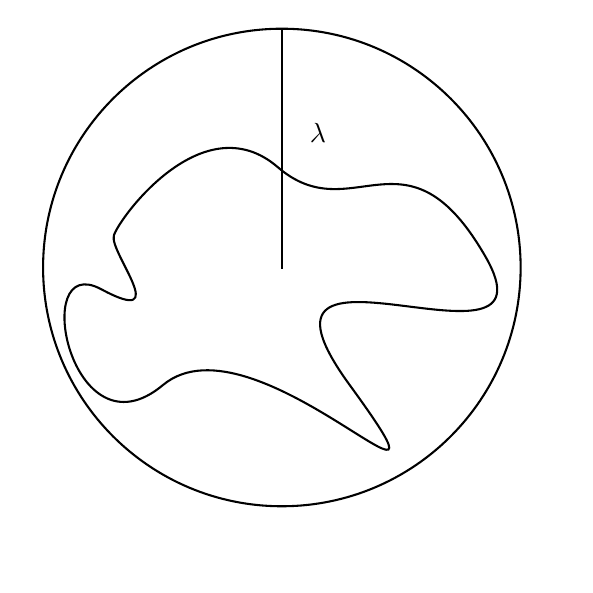
\begin{tikzpicture}[x=0.75pt,y=0.75pt,yscale=-1,xscale=1]

\draw   (266.34,108.02) .. controls (268.59,99.95) and (309.34,44.02) .. (345.34,75.02) .. controls (381.34,106.02) and (407.34,52.02) .. (445.34,118.02) .. controls (483.34,184.02) and (317.34,94.02) .. (380,180) .. controls (442.66,265.98) and (334.34,143.02) .. (290,180) .. controls (245.66,216.98) and (225.34,115.02) .. (260.26,133.81) .. controls (295.19,152.61) and (264.09,116.08) .. (266.34,108.02) -- cycle ;
\draw   (232.26,123.35) .. controls (232.26,59.82) and (283.77,8.31) .. (347.3,8.31) .. controls (410.84,8.31) and (462.34,59.82) .. (462.34,123.35) .. controls (462.34,186.88) and (410.84,238.39) .. (347.3,238.39) .. controls (283.77,238.39) and (232.26,186.88) .. (232.26,123.35) -- cycle ;
\draw    (347.3,8.31) -- (347.3,124.02) ;

\draw (359.33,52.4) node [anchor=north west][inner sep=0.75pt]    {$\lambda$};

\end{tikzpicture}

\end{figure*}

\begin{theorem}{
	Given $S$ is a compact subset of $X$ and $f:X\to\r$ is continuous, then $f$ has a maximum point in $S$.
}
	Since $S$ is compact and $f$ is continuous, $f(S)$ is compact.
	Hence $f(S)$ is closed and bounded.
	Let
	\[
		\alpha \coloneqq \sup(f(S)).
	\]
	Then $\alpha\in f(S)$ since $f(S)$ is closed.
	So there exists $x_0\in S$ such that
	\[
		f(x_0) = \alpha.
	\]
	Therefore $f$ attains a maximum on $S$.
\end{theorem}

\begin{theorem}{
	If $f:X\to Y$ is continuous and $A$ is a compact subset of $X$, then $f$ is uniformly continuous on $A$.
}
	Let $\eps > 0$.
	For each $p\in A$, there exists $\delta_p > 0$ such that
	\[
		d_X(p,x) < \delta_p \implies d_Y(f(p),f(x)) < \frac{\eps}{2}.
	\]
	Consider the open cover
	\[
		\{\vee_{\delta_p/2}(p) : p\in A\}.
	\]
	By compactness, there is a finite subcover
	\[
		\{\vee_{\delta_{p_i}/2}(p_i) : 1 \leq i\leq N\}.
	\]
	Choose
	\[
		\delta \coloneqq \min_{1\leq i\leq N}\frac{\delta_{p_i}}{2}.
	\]
	We show that
	\[
		d_X(x,y) < \delta \implies d_Y(f(x),f(y)) < \eps
	\]
	for all $x,y\in A$.
	Given $x\in A$, choose $p_i$ such that
	\[
		x\in \vee_{\delta_{p_i}/2}(p_i).
	\]
	So
	\[
		d_X(x,p_i) < \frac{\delta_{p_i}}{2}.
	\]
	If also $d_X(x,y) < \delta$, then
	\[
		d_X(x,y) < \frac{\delta_{p_i}}{2}.
	\]
	By the triangle inequality,
	\[
		d_X(y,p_i) \leq d_X(y,x) + d_X(x,p_i) < \frac{\delta_{p_i}}{2} + \frac{\delta_{p_i}}{2} = \delta_{p_i}.
	\]
	Hence both $x$ and $y$ lie in $\vee_{\delta_{p_i}}(p_i)$.
	Therefore
	\[
		d_Y(f(x),f(p_i)) < \frac{\eps}{2}
		\qquad\text{and}\qquad
		d_Y(f(y),f(p_i)) < \frac{\eps}{2}.
	\]
	So
	\[
		d_Y(f(x),f(y)) \leq d_Y(f(x),f(p_i)) + d_Y(f(p_i),f(y)) < \eps.
	\]
	Thus $f$ is uniformly continuous on $A$.
\end{theorem}